% Une ligne commentaire débute par le caractère « % »

\documentclass[a4paper]{article}

% Options possibles : 10pt, 11pt, 12pt (taille de la fonte)
%                     oneside, twoside (recto simple, recto-verso)
%                     draft, final (stade de développement)

\usepackage[utf8]{inputenc}   % LaTeX, comprends les accents !
\usepackage[T1]{fontenc}      % Police contenant les caractères français
\usepackage[francais]{babel}
\usepackage{fullpage}
\usepackage{multicol}
\usepackage[colorlinks=true,linkcolor=blue,urlcolor=black,bookmarksopen=true]{hyperref}
\usepackage{bookmark}
\usepackage{blindtext}



\usepackage{graphicx}  % pour inclure des images
\graphicspath{ {rapport/img/} }

%\pagestyle{headings}        % Pour mettre des entêtes avec les titres
                              % des sections en haut de page

 \title{  TP1 : Les Bases d'Android\\         % Les paramètres du titre : titre, auteur, date
  Programmation mobile}
\author{Mohamad Satea Almallouhi - Tony Nguyen\\
  \emph{M1 Génie Logiciel}\\
  Faculté des Sciences\\
Université de Montpellier.}
\date{27 Février 2024}



\begin{document}
\maketitle                    % Faire un titre utilisant les données
                              % passées à \title, \author et \date

\begin{center}
  
\includegraphics[scale=1]{cuteGirl.jpeg}
\end{center}

% \begin{abstract}     % Résumé du travail

%   \emph{Description très succinte du problème et des différentes étapes de réalisation}

% \end{abstract}
\newpage
%\dominitoc  % initializer les minitoc
\tableofcontents
\section*{Introduction}
  \paragraph{}
    Dans ce TP, nous allons voir les bases de la programmation mobile pour Android en Java.
  
    Les sections de rapport suit les exercices.
    Les sections de rapport suit les exercices. Les sections de rapport suit les exercices. Les sections de rapport suit les exercices. Les sections de rapport suit les exercices.
    
    Les sections de rapport suit les exercices.
    Les sections de rapport suit les exercices. Les sections de rapport suit les exercices. Les sections de rapport suit les exercices. Les sections de rapport suit les exercices.


  \paragraph{}

    Les sections de rapport suit les exercices.
    Les sections de rapport suit les exercices. Les sections de rapport suit les exercices. Les sections de rapport suit les exercices. Les sections de rapport suit les exercices.

    Les sections de rapport suit les exercices.
    Les sections de rapport suit les exercices. Les sections de rapport suit les exercices. Les sections de rapport suit les exercices. Les sections de rapport suit les exercices.


    Les sections de rapport suit les exercices.
    Les sections de rapport suit les exercices. Les sections de rapport suit les exercices. Les sections de rapport suit les exercices. Les sections de rapport suit les exercices.

\newpage

\begin{multicols}{2}
  [
    Faire une vidéo, rapport+read.md(instruction) screenchot résultats + code. +bonus bien fait,beau,tests,Kotlin,latex
  \section{Hello world}
  Nous allons voir comment afficher du texte à l'écran dans une activité sa vue associé.
  ]
  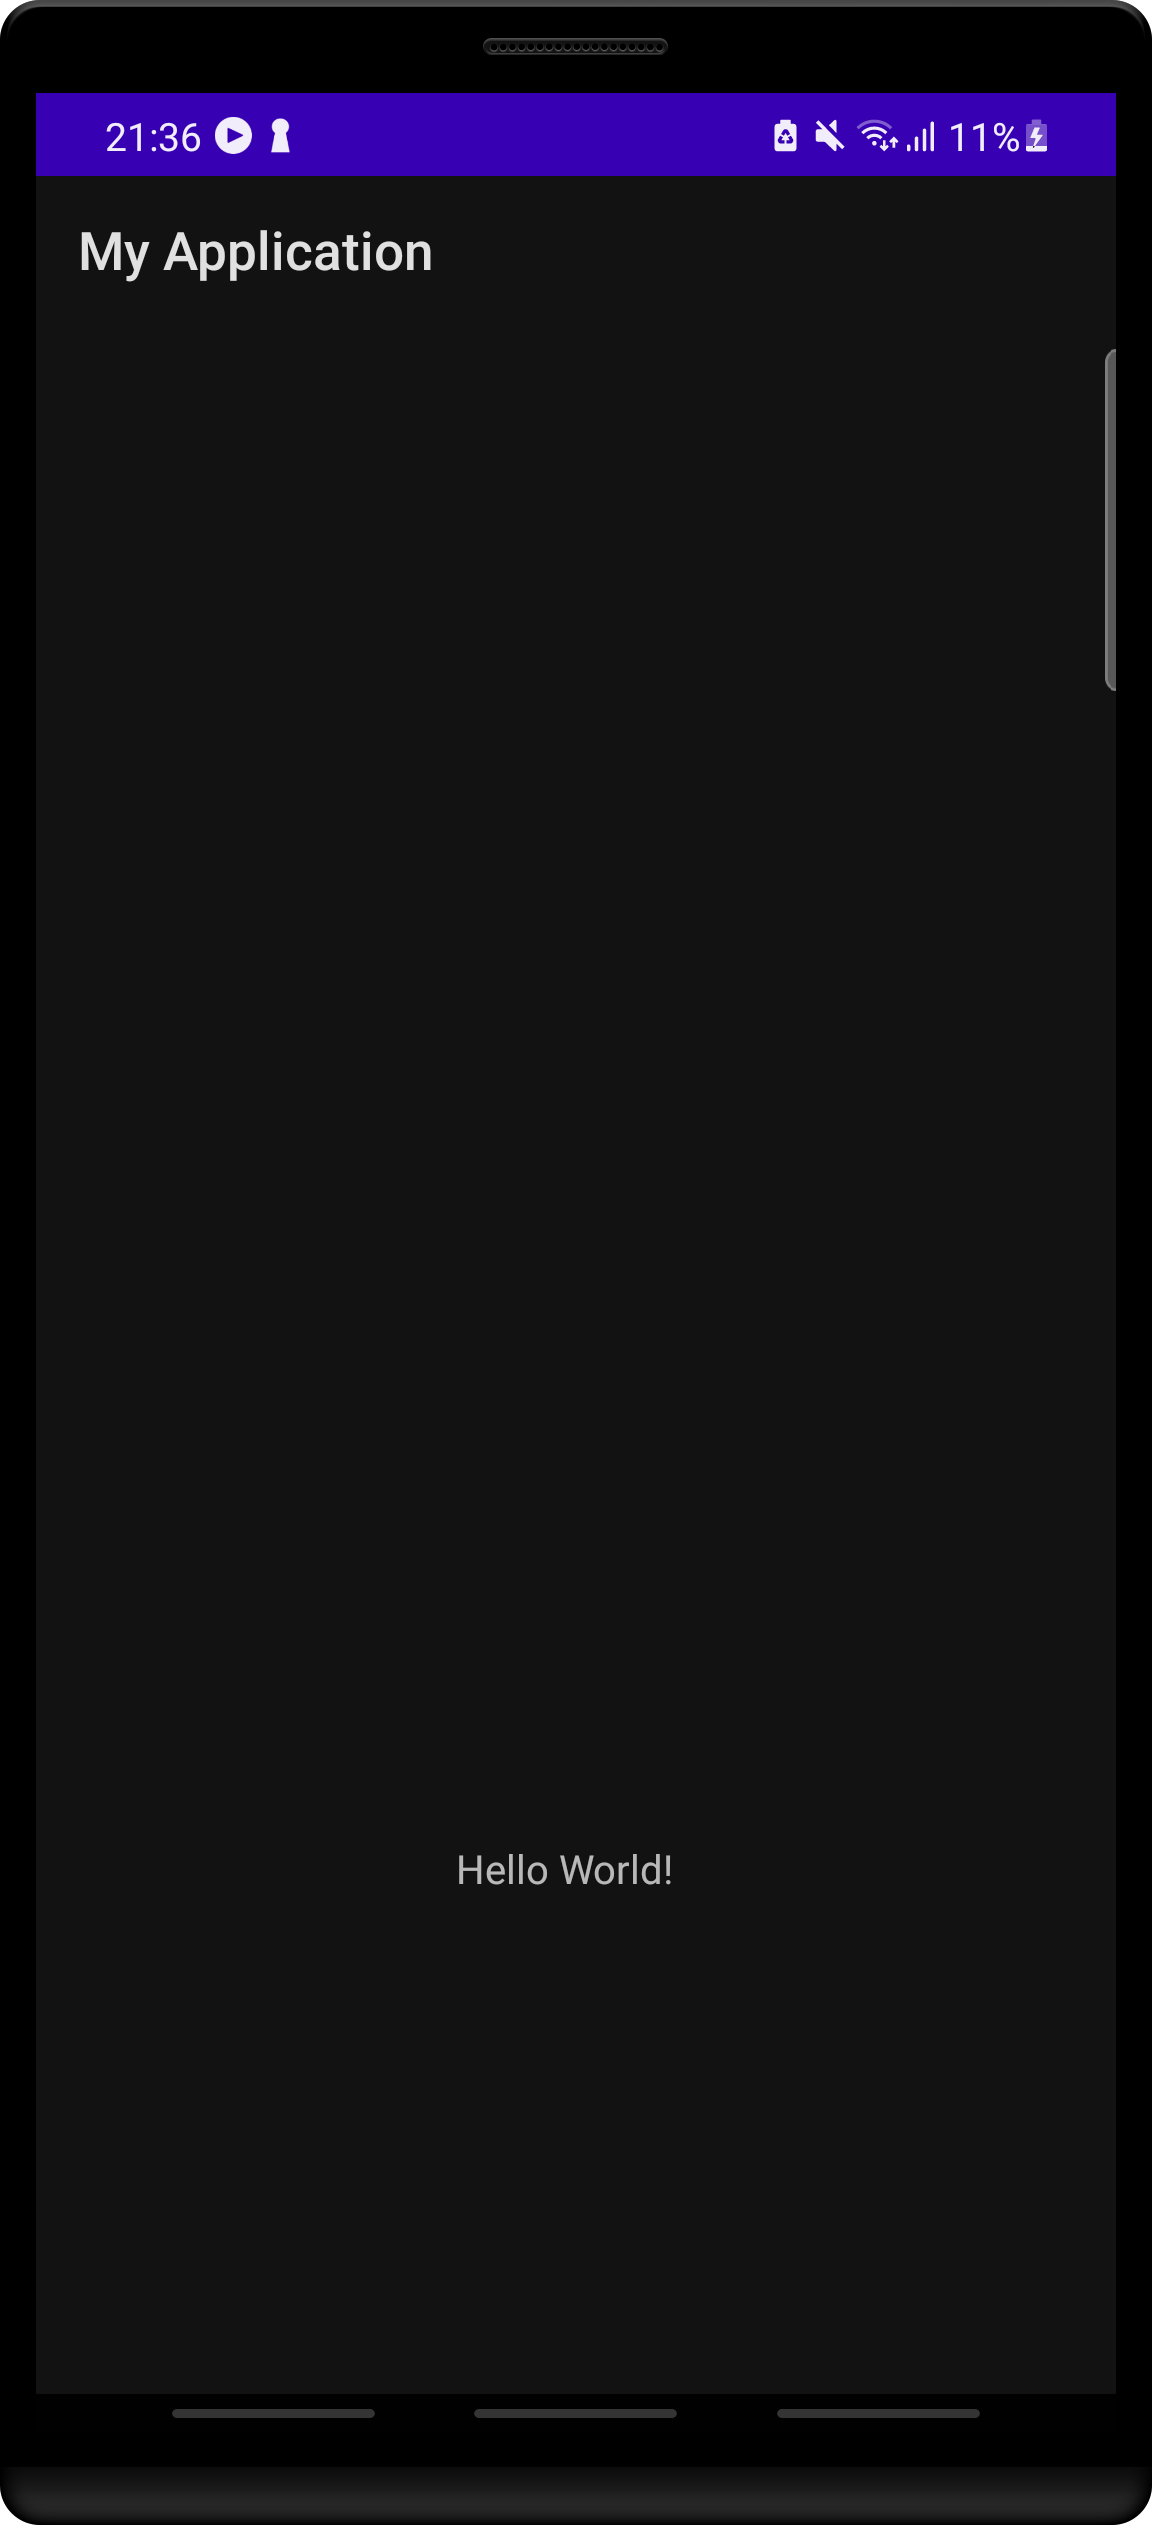
\includegraphics[height=0.9\textwidth]{captureHelloWorldAppPhone}
  \paragraph{}
  Tout d'abord, dans un fichier .xml dans res/layout, nous déclarons une balise \textbf{<TextView>} avec un attribut \textbf{android:text} qui a pour valeur "Hello World!".
  \newline\newline
  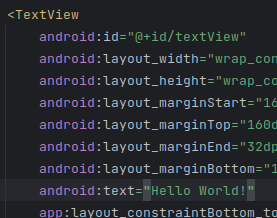
\includegraphics[width=.49\textwidth]{screenshotHelloWorldLayout}
  % 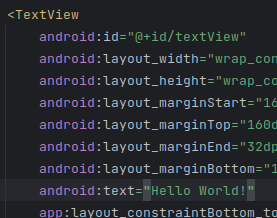
\includegraphics[width=.457\textwidth]{screenshotHelloWorldLayout}
  \newline
  
  Afin de l'afficher à l'écran on va utilser ce \textbf{layout} dans une activité à l'aide de la fonction \textbf{setContentView()}.
  \newline

  Il est également nécessaire d'indiquer à l'application l'activité à lancer comme point d'entrée. Pour cela, dans le manifest, nous ajoutons la balise \textbf{<intent-filter>}, voir figure \ref{fig:manifestHelloWorld} (page \pageref{fig:manifestHelloWorld}) pour plus de détail.
  \newline
  \newline
  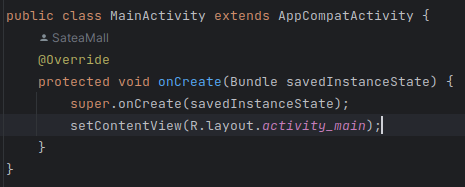
\includegraphics[width=0.49\textwidth]{screenshotCodeHelloWorld.png}
% \end{multicols}
\begin{figure*}
  \centering
  \caption{Manifest pour l'application HelloWorld}
  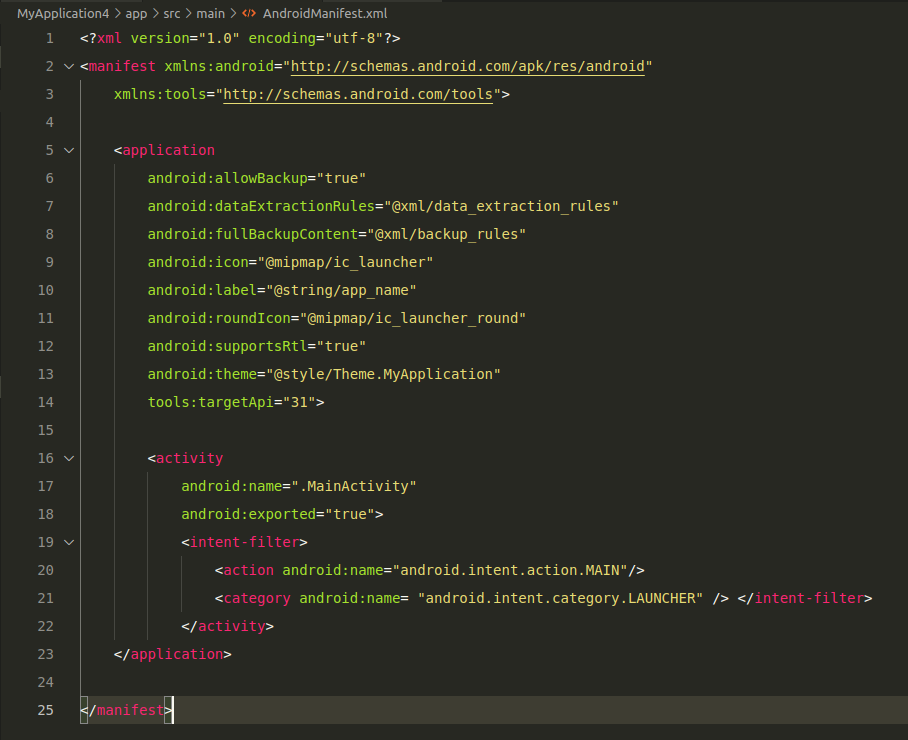
\includegraphics[width=.7\textwidth]{screenshotHelloWorldManifest.png}
  \label{fig:manifestHelloWorld}
\end{figure*}
\section{Simple formulaire}
% \begin{multicols}{2}
  
  \paragraph{}
  Nous allons voir comment faire une application android réalisant un formulaire où l'on demandera des informations de différentes nature à l'utilisateur.
  
  % \begin{figure*}[t]
  %   \centering % à mettre avant includegraphics
  %   
\includegraphics[scale=0.5]{cuteGirl.jpeg}
  %   \caption{Very cute anime girl}
  % \end{figure*}
  \subsection{Internationalisation}
  Utilisation de ressources R
  
  Utilisation du concept de ressources. Dans res/values/strings.xml, nous déclarons les différents valeurs, mais avec le même attribut name.
  
  \subsection{Évenements}
  
    \paragraph{}
      Test Test Test Test Test Test Test Test Test Test Test Test Test Test Test Test 

      Beep boop. Beep boop. Beep boop. Beep boop. Beep boop. Beep boop. 
    \paragraph{}
      Test Test Test Test Test Test Test Test Test Test Test Test Test Test 
  
  \subsection{Intent explicite}
    Qu'est ce qu'un "Intent" ? 
    
    
    \subsection{Intent implcite}
      beep boop

  \section{Consultation les horaires de trains}
    \paragraph{}
      Nous allons faire une application pour consulter des horaires de trains.
    \begin{figure*}
      \centering
      \caption{Diagramme de classe de l'application Trains}
      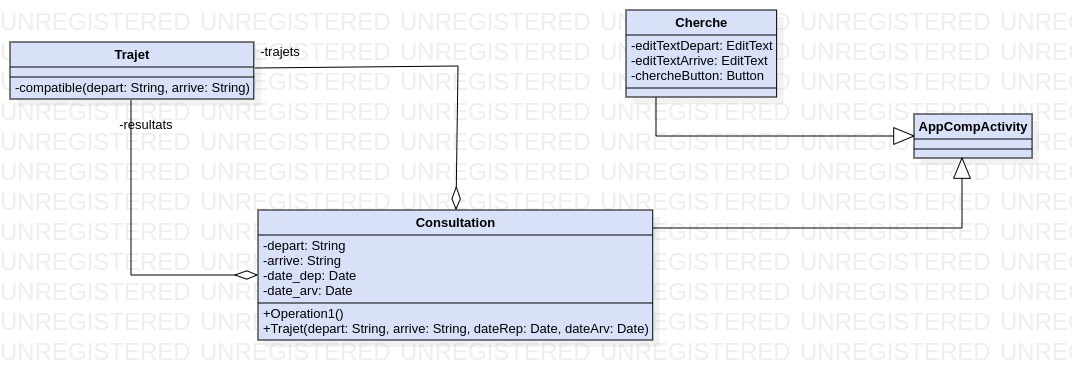
\includegraphics[width=\textwidth]{jpg/Model1!Train_1}
      \label{fig:manifestHelloWorld}
    \end{figure*}
  \section{Simple d’agenda}
    \paragraph{}
      Nous allons réalisé une application d'agenda.
    \begin{figure*}
      \centering
      \caption{Diagramme de classe de l'application Agenda}
      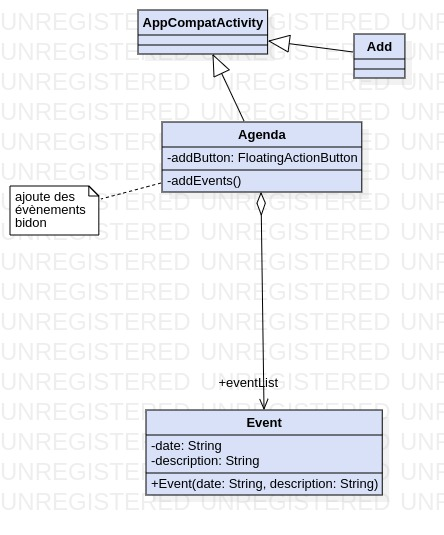
\includegraphics[width=\textwidth]{jpg/Model!Agenda_0}
      \label{fig:manifestHelloWorld}
    \end{figure*}
  \end{multicols}
\end{document}